\documentclass{article}

% if you need to pass options to natbib, use, e.g.:
%     \PassOptionsToPackage{numbers, compress}{natbib}
% before loading neurips_2022

% ready for submission
\usepackage[preprint]{neurips_2022}

% to compile a preprint version, e.g., for submission to arXiv, add add the
% [preprint] option:
%     \usepackage[preprint]{neurips_2020}

% to compile a camera-ready version, add the [final] option, e.g.:
%     \usepackage[final]{neurips_2020}

% to avoid loading the natbib package, add option nonatbib:
%\usepackage[nonatbib]{neurips_2020}
\usepackage[utf8]{inputenc} % allow utf-8 input
\usepackage[T1]{fontenc}    % use 8-bit T1 fonts
\usepackage{hyperref}       % hyperlinks
\usepackage{url}            % simple URL typesetting
\usepackage{booktabs}       % professional-quality tables
\usepackage{amsfonts}       % blackboard math symbols
\usepackage{nicefrac}       % compact symbols for 1/2, etc.
\usepackage{microtype}      % microtypography


% Graphics and color
\usepackage{graphicx}
\usepackage{xcolor}

% References and Bibliography
\usepackage{url}
\usepackage{hyperref}
\hypersetup{
  colorlinks,
  linkcolor={black},
  citecolor={blue!50!black},
  urlcolor={blue!50!black}
}
\usepackage{cleveref}
\usepackage[numbered]{bookmark} % Fixes false PDF table of contents
\usepackage{natbib}
\setcitestyle{numbers,sort&compress,square,comma}
\usepackage{bibentry}
\nobibliography*

\title{Impact of most Common Food Categories on\\ Green House Gas Emissions}


\author{%
  Hanna Dettki\thanks{Equal contribution.} \\
  Department of Computer Science\\
  University of Tübingen\\
  \texttt{hanna.dettki@student.uni-tuebingen.de} \\
  \And
  Davide $^{*}$  \\
  Department of Computer Science\\
  University of Tübingen\\
  \texttt{@student.uni-tuebingen.de} \\
  % \AND
  % Coauthor \\
  % Affiliation \\
  % Address \\
  % \texttt{email} \\
  % \And
  % Coauthor \\
  % Affiliation \\
  % Address \\
  % \texttt{email} \\
  % \And
  % Coauthor \\
  % Affiliation \\
  % Address \\
  % \texttt{email} \\
}

\begin{document}

\maketitle

\begin{abstract}
  This research is made for the Data Literacy Project of the academic year 2022/2023. It covers the discussion about the emissions of a plant based diet in comparison with a traditional diet. The research is conducted by exploration of the data, hypothesis testing and example comparisons. 
\end{abstract}

\section{Introduction}

Climate change threatens everyone. In order to avoid a climate disaster, radical change is needed. This concerns everything, from policies on a global and national level, to choices taken by the individual on a daily basis. 
However, individuals motivated and willing to solve climate change by pursueing a sustainable life are faced with many obstacles to do so effortlessly. Food, energy and water is what the UN refer to as the culprit for a sustainable world, who's population has expanded and who's demand has increased for  all three of the aforementioned  \cite{Ritchie2020}.
 Importantly, food systems are responsible for a third of global anthropogenic greenhouse gas emissions \cite{Crippa2021}. At the same time, food choices are to a large extent up to the individuum.  Tragically,  the emission of food options are not handily accessible to the individuum, which is why one is not able to take an informed climate friendly food decision. This shows that a significant lever contributing to solving climate change is not pulled!
\paragraph*{Research Question}
Therefore, we investigate the environmental impact of the most common food categories, which is a first step towards  providing more information in the jungle of food choices that everybody is presented with. In particular, we hypothesize that  plant-based diets  have a significantly smaller CO$_2$-footprint than  diets including animal-derived products in the typical Western diet. .

\section{Data}
\label{data}
\paragraph{Data generating process} \label{dataGen}
The data used in this analysis  is the largest meta-analysis of food systems to date and was published in the journal \textit{Science} by \citet{Poore2018}.
570 studies met the eleven criteria\footnote{Such as  methodologies used were standardized, e.g., that all stages of the supply chain were considered.} \citet{Poore2018}  were applying to the initially  1530 studies.
The final dataset covers approximately 38,700 farms across 119 countries and spans a total of 40 food products, which represent approximately 90\% of global protein and calorie intake. The breadth of this analysis ensures that results are only minimally biased towards any geographic region, or are reflective of any particular faming method or income level.
\paragraph*{Greenhouse gases (GHG) and how they are quantified}
Since there are many different greenhouse gases (GHG), researchers commonly aggregate them into a measurement that is easy to use for comparisons. 
\citet{Poore2018} use the metric 
''carbon dioxide-equivalents (CO$_{2}$eq)'', which is the most common measurement and is for instance  also used as a target-setting metric in official reportings like the Paris Agreement. CO$_{2}$eq express the "global warming potential" by aggregating the impact of all GHG into a single metric  and  aims to represent the amount of warming that each specific gas generates relative to CO$_2$. The "global warming potential over a $100$-year timescale (GWP$_{100}$) expresses the mid- to longterm period for climate-policies. CO$_{2}$eq is calculated as follows: 
\paragraph{Stages of supply chain}
Note: only if included in analysis
% Land use change; 
% On-farm impacts in crop or livestock production (including the manufacturing of inputs such as fertilizers, or emissions from manure);
% Animal feed production;
% Food processing: the conversion of raw ingredients into sold products, such as the processing of cereals into bread;
% Transport: this includes transport from the farm up to retail. Transport of food from retail to consumers’ homes is not included.
% Packaging
% Retail: energy consumption in retail stores, such as refrigeration.



\paragraph{Dataset adaptions and handling of missing data}

We substituted  missing  data by taking the mean of the existing values of the respecting feature. To facilitate data queries, we added a column "Plant-based", which holds binary values $[0,1]$ and indicates whether a product is plant-based $(1)$ or animal-derived $(0)$.


\section{Analysis}
\label{analysis}


\begin{figure}[h]
  \centering
  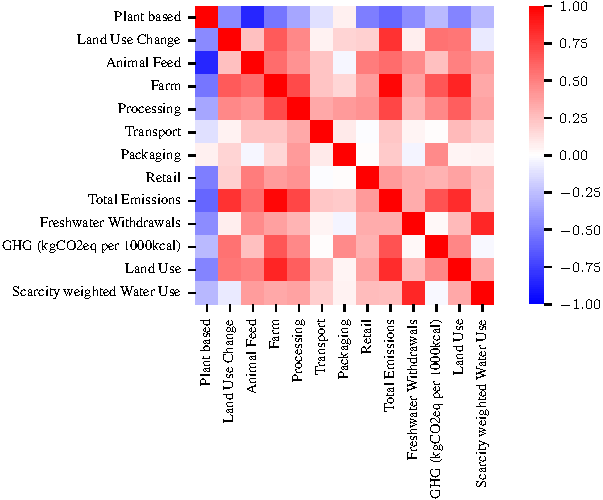
\includegraphics[width=0.75\textwidth]{figures/heat-map.pdf}
  \caption{Some caption text.}
\end{figure}

\subsection{Average Emissions for Plant-based and Animal-based Products}
\paragraph{Eutrophying emissions}
\paragraph{Accounting  for Nutritional Value}
\paragraph{Comparing Typical Diets}

\section{Conclusion}
\label{conclusion}


\section{Limitations}
\label{limitations}

\subsection{Tables}



Note that publication-quality tables \emph{do not contain vertical rules.} We
strongly suggest the use of the \verb+booktabs+ package, which allows for
typesetting high-quality, professional tables:
\begin{center}
  \url{https://www.ctan.org/pkg/booktabs}
\end{center}
This package was used to typeset Table~\ref{sample-table}.

\begin{table}
  \caption{Sample table title}
  \label{sample-table}
  \centering
  \begin{tabular}{lll}
    \toprule
    \multicolumn{2}{c}{Part}                   \\
    \cmidrule(r){1-2}
    Name     & Description     & Size ($\mu$m) \\
    \midrule
    Dendrite & Input terminal  & $\sim$100     \\
    Axon     & Output terminal & $\sim$10      \\
    Soma     & Cell body       & up to $10^6$  \\
    \bottomrule
  \end{tabular}
\end{table}


\section*{Broader Impact}

\begin{itemize}
\item reducing GHG
\item animal welfare
\item biodiversity
\item Health: While there are some concerns, that vegan diets (i.e, plant-based diets that exclude all forms of animal products in their entirety) are not sufficient w.r.t providing recommended micronutiernt levels (e.g. vitamin B12, zinc, iron, etc.), they generally meet protein intake recommendations. Nonetheless, individuals who consume a vegan diet should remain aware regarding potential micronutirent insufficiencies. 
\end{itemize}



\section*{Literature}

List of selected central research literature that the project is based on.


\begin{itemize}
  \item \bibentry{Ritchie2020}
  \item \bibentry{Michigan2021}
  \item test \citet{WHO2021}
\end{itemize}

\subsection{Related Literature}
\begin{itemize}
  \item \bibentry{Pieper2020}
  %\item \bibentry{Felix2021}
\end{itemize}


{\small
\bibliographystyle{unsrtnat}
\bibliography{../literature/references.bib}
}
\end{document}
